\section{Durchführung}
\subsection{Aufbau}
\label{sec:Durchführung}
Der Aufbau besteht hauptsächlich aus einer optischen Strecke. Das Licht einer Spektrallampe wird gebündelt und auf $\lambda = \SI{794,8}{\nano \meter}$
gefiltert. Das entspricht der $\text{D}_1$ Linie von Rubidium, welches untersucht wird. Mit einer Kombination aus einem Polarisationsfilter und einer
$\sfrac{\lambda}{4}$-Platte wird das Licht rechtszirkular polarisiert. Dieses Licht durchquert eine Dampfzelle, in der eine Mischung aus den Rubidium-Isotopen ${}^{87}\text{Rb}$
und ${}^{87}\text{Rb}$ gasförmig vorliegt. Die Dampfzelle ist beheizt, um einen optimalen Dampfdruck zu erzeugen. Das austretende Licht wird gebündelt
und von einem Photoelement gemessen. Die optischen Bauteile werden so justiert, dass die Intensität am Photoelement maximal ist. Die Dampfzelle ist von drei Helmholtzspulen umgeben, von denen eine zum Ausgleich des Erdmagnetfeldes ist und zwei für
die Erzeugung der Zeeman-Niveaus. Dieser Aufbau ist in Abbildung \ref{fig:aufbaucom} skizziert.


\begin{figure}
	\centering
	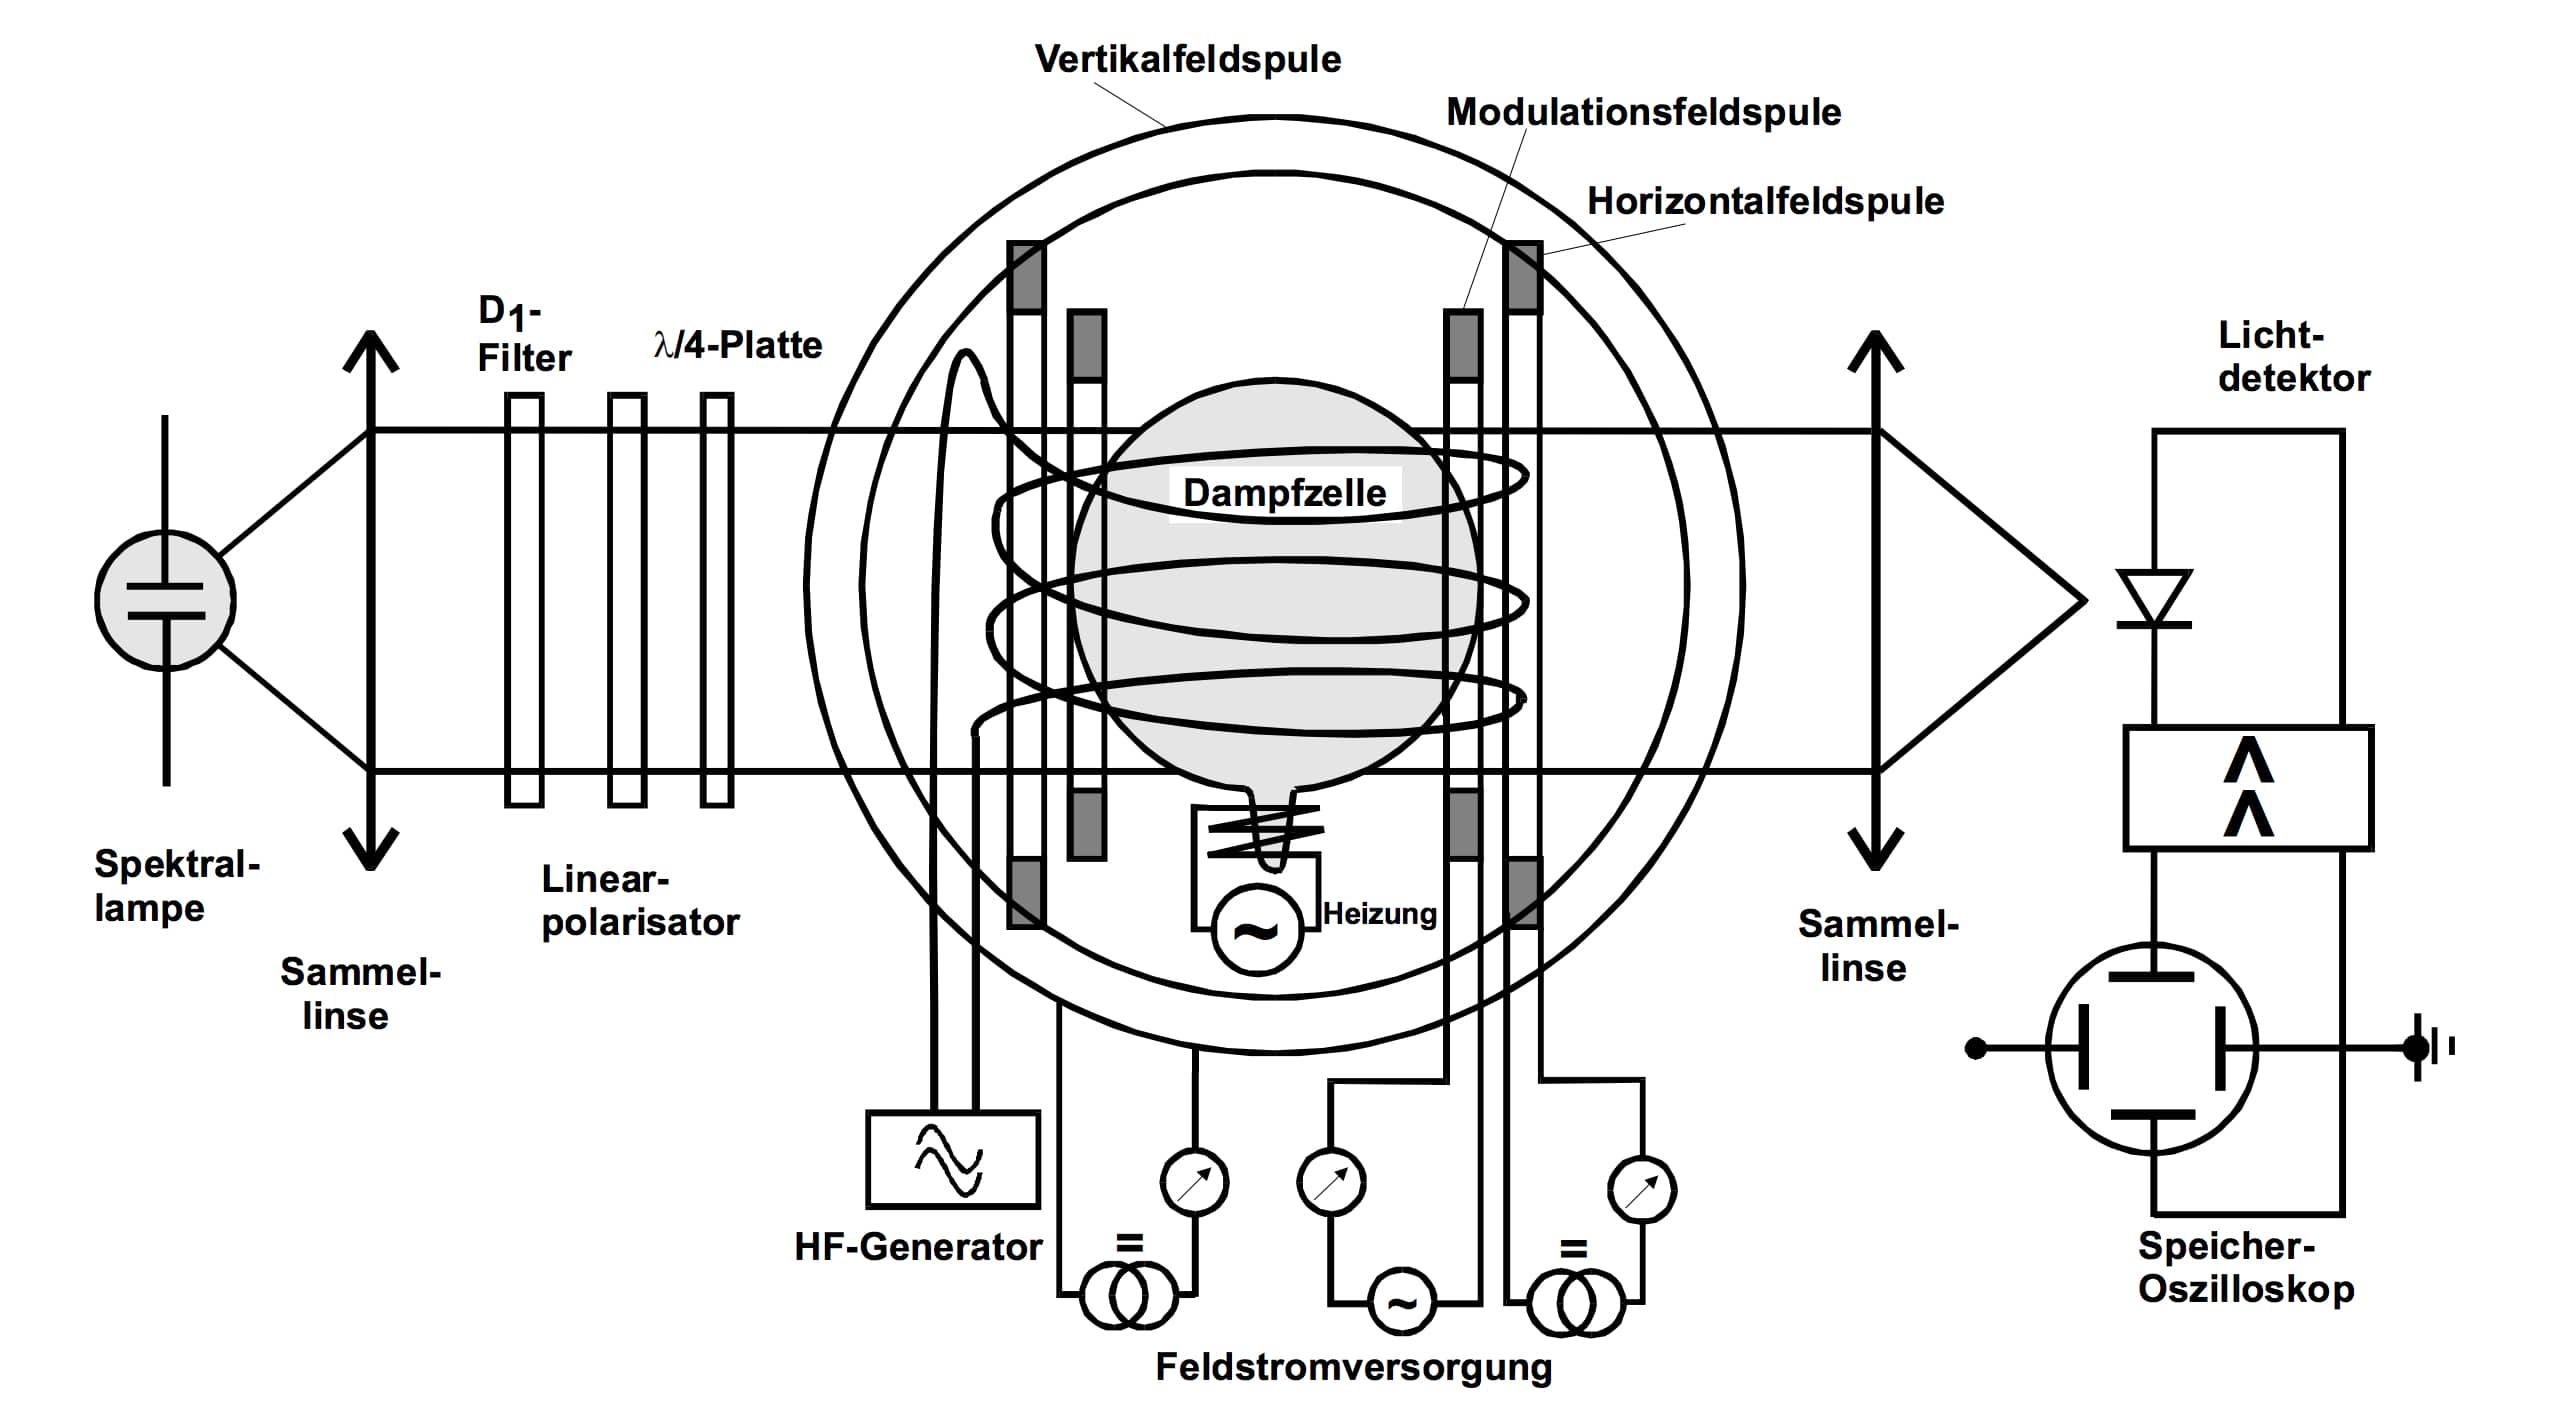
\includegraphics[width=0.8\linewidth]{img/aufbaucom.jpg}
	\caption{Schematischer Aufbau des optischen Pumpens.\cite{V21}}
	\label{fig:aufbaucom}
\end{figure}

\subsection{Kompensation des Erdmagnetfelds}
Zunächst muss der Aufbau so gedreht werden, dass er parallel zu der Horizontalkomponente des Erdmagnetfelds steht. Als nächstes wird dessen Vertikalkomponente ausgeglichen. Dazu wird zunächst die Photodiode mit dem Kanal 2 des Oszilloskops verbunden. Auf Kanal 1 wird der Recorder-Ausgang der Sweepspule gelegt und das Oszilloskop wird auf XY Betrieb gestellt. Auf dem Oszilloskop ist nun ein breiter nach unten gerichteter Peak zu sehen. Dieser wird mithilfe der Vertikalspule auf minimale Breite gebracht. Das Nulldurchgang-Minimum entsteht durch die bei verschwindendem Magnetfeld fehlende Zeeman-Aufspaltung, wodurch kein optisches Pumpen möglich ist und die Transparenz minimal wird.

\begin{figure}[h]
	\centering
	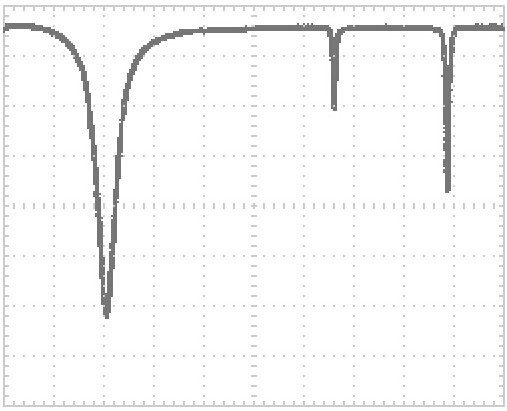
\includegraphics[width=0.7\linewidth]{img/oszi1_2}
	\caption{Typische Aufnahme auf dem Oszilloskop bei einer Frequenz von $\SI{100}{\kilo \hertz}$. Aufgetragen ist die Transparenz des Rubidiumdampfes in Abhängigkeit vom angelegten Magnetfeld. Die drei Minima entsprechen von links nach rechts einem verschwindenden Magnetfeld und den Resonanzstellen der beiden Rubidium-Isotope beim optischen Pumpen.}
	\label{fig:oszi1_2}
\end{figure}

\subsection{Vermessung der Resonanzstellen}
Zur Vermessung weiterer Resonanzstellen wird die Frequenz der RF-Spule von $\SI{100}{\kilo \hertz}$ bis $\SI{1}{\mega \hertz}$ in $\SI{100}{\kilo \hertz}$-Schritten erhöht, wobei in jedem Schritt der Strom gemessen wird, bei dem die Resonanzen auftreten. In Abbildung \ref{fig:oszi1_2} ist eine typische Aufnahme eines Sweep-Durchgangs bei einer Frequenz von $\SI{100}{\kilo \hertz}$ zu sehen. Die Ordinate ist proportional zur Transparenz des Rubidiumdampfes für das eingestrahlte rechtszirkular polarisierte Licht und die Abszisse ist proportional zum Magnetfeld, welches durch die beiden horizontalen Spulen erzeugt wird. Die zu beobachtenden Minima in der Transparenz entsprechen von links nach rechts dem Nulldurchgang des Magnetfelds, der Resonanzstelle des ersten Rubidium-Isotops und der Resonanzstelle des zweiten Rubidium-Isotops. Beim verschwindenden Magnetfeld ist die Transparenz des Dampfes am geringsten, da dann keine Zeeman-Aufspaltung der Energieniveaus auftritt und somit kein optisches Pumpen möglich ist. Um das Verhältnis der Rb-Isotope zu bestimmen, wird ein Bild des Oszilloskops aufgenommen, auf dem die zwei Dips der Transparenz zu sehen sind. 

